\documentclass{article}[12pt]

\usepackage{amsmath}
\usepackage{graphicx}

\author{zlyu0226}
\title{COMP5329: Assignment1\\Report}

\begin{document}
\maketitle

\section{Introduction}\label{sec:introduction}
\subsection{Aim of study}\label{subsec:aim-of-study}
    The aim of this study is to understand the fundamentals of deep learning by implementing
    simple multilayer perceptron neural networks and related functions such as optimizers,
    activation functions and loss functions.
\subsection{Importance of study}\label{subsec:importance-of-study}
    The importance of this study is that the best way to learn the principles of deep
    learning is to practice them.

    However, mature frameworks often hide the process and methods of implementation
    from the user, wrapping complex processes in simple interfaces.Calling these
    encapsulated interfaces does not allow people to understand the principles,
    but merely to become "skilled interface users".
    Once a problems arises, When a problem arises, those who do not understand
    the principles are often unable to locate the root cause of the problem,
    or to deduce how to optimise the model by modifying hyperparameters.

    In this study, by implement an independent deep learning framework, subjects will obtain a
    better understanding towards the underlying principle of deep learning, and thus become a better
    problem solver in deep learning area.

\section{Methodology}\label{sec:methodology}
\subsection{Preprocessing}\label{subsec:preprocessing}
\subsubsection{Data Overview}\label{subsubsec:data-overview}
    The given data set is in shape of $(50000, 128)$, with a label of single integer value (0-9).
    The feature data has a standard deriviation of $1.1688637$ and mean $-1.59374025$.
    From the data quality perspective, the standard deriviation is very close to 1 and mean is close to 0,
    which is pretty good for model training.

    For the label data, the ground truth of samples are perfectly distributed.
    There are 10 classes in total, $50000$ samples, and $5000$ samples for each class precisely.

\subsubsection{Preprocess the Feature Data}
    Although the standard deriviation and mean of the feature data is good, there is still room for improvement.
    Before training, the feature data was standardized to 0 mean and standard deriviation 1 using the following method:
\[ x_{Standardized} = \frac{x - \mu}{\sigma} \]
    Where $\mu$ stand for mean of x and $\sigma$ is the standard deriviation of x.

\subsubsection{Preprocess the Label Data}
    The label data is in form of (0-9), which is numerically continuous but discrete in meaning.
    To make it able to be feed into the model, it must be encoded.
    Before training, the label data was one hot encoded from single integer to a 10 element vector.
    For example:

    \[ OnehotEncode([0, 1, 2]) = [[1, 0, 0], [0,1,0],[0,0,1]] \]

\subsection{Design}
    The best model is designed with 3 hidden layer, with 64, 32, 10 neuron seperately, initialized by
    Xavier Normal initialization.
    Each hidden layer is followed by a batch-normalization layer and a dropout layer with drop rate 0.25.
    Activation function is ReLU. Specifically, for last layer, the activation function is Softmax.
    Optimizer is Adam with momentum $\beta_1 = 0.9$ $\beta_2 = 0.999$,
    learning rate $1e-3$ and weight decay $0.02$.
    Loss function is Cross Entropy.

\subsection{Module}
\subsubsection{Layer}
    In a multilayer perceptron, the hidden layer is the fully connected layer.
    Its role is to take the features of the input data and abstract them into another dimensional space
    to reveal its more abstracted features, which can be better divided linearly.
    Multiple hidden layers are multiple levels of abstraction of the input features to achieve a better linear division.

    The layer keeps multiple neurons, each one contains two variable, weight and bias.
    Each neuron for each input $X$, it does:
\[ w^T X+b\]
    For a well-trained model, each neuron can be activated by a specific combination of features,
    outputting a strong signal to the next layer, thus contributing to the final result.

\subsubsection{Batch-normalization}
    Batch-normalization layer is to normalize the batch data during the training process.
    This layer will compute a moving average of mean and standard deriviation of output from previous layer,
    and normalize them to reach 0 mean and 1 standard deriviation.

\begin{gather*}
    \mu_{t} = \mu_{t-1} * (1-momentum) + momentum *\mu\\
    \sigma_{t} = \sigma_{t-1} * (1-momentum) + momentum *\mu\\
    Normalized_{t} = \frac{input_{t} - \mu_{t}}{\sigma_{t}}
\end{gather*}

    After normalization, the batchNorm layer will also do a shifting like hidden layer:

\[ out_{t} = \gamma Normalized_{t} + \beta \]

    Where $\gamma$ and $\beta$ are also trainable.

\subsubsection{Dropout}
    The dropout layer is used to make the output of the hidden layer sparse and reduce the complex co-adaptation
    relationship between neurons, thus reducing the probability of overfitting the model.

    The principle of it is to randomly set neurons' output to zero.
    The probabilty of this zerolization is user-defined.

\subsubsection{ReLU}
    ReLU, Rectified Linear Unit, is a kind of activation.
    It works by non-linearly transforming the linear output of each layer, so that the whole model becomes non-linear
    and more complex decision boundaries can be formed.

    It works by zeroing out negative numbers in the output of the previous layer,
    leaving values greater than or equal to zero as they are.

\subsubsection{Softmax}
    Softmax maps some inputs to real numbers between 0 and 1, and normalizes them to ensure that the sum is 1.
    It is designed to be used for multiple classification tasks, since the probability of multiple classes also sums to 1.

    For the input $V = [V_1, V_2, \dots V_j]$:
\[ Out_i = \frac{e^{V_i}}{\Sigma^i_j e^{V_i}}\]

\subsubsection{Adam}
    Adam optimization is a stochastic gradient descent method that is based on adaptive estimation of first-order and
    second-order moments.
    Effective control of the learning rate step and gradient direction through first and second order momentum,
    preventing oscillation of the gradient and stationarity at the saddle point.

    If weight decay is defined, the gradient will be added by the $W * decayRate$ before updating.

\[g_t = g_t + W_{t-1} * decayRate\]

    First order moment: a moving average of gradient.

\[m_t = \beta_1 * m_{t-1} + (1 - \beta_1) * g_t\]

    Second order moment: a moving average of squared gradient.

\[V_t = \beta_2 * V_{t-1} + (1 - \beta_2) * g_t^2\]

    After the moments were computed, update the variable

\[W_t = W_{t-1} - \frac{lr * m_t}{\sqrt{V_t}}\]

\subsubsection{CrossEntropy}
    CrossEntropy loss function is designed to evaluate the prediction performance in multi-classification task.
    Its derivative is directly depends on the prediction and ground truth, thus it will be a very good loss function
    when the model is performing bad.
    But for a better model, the learning speed will decrease.

    For prediction $p$ and ground truth $y$:

\[ L = \frac{1}{N} \sum_i L_i  = -\frac{1}{N}\sum_i \sum^M_{c=1} y_{ic} \log(p_{ic}) \]

    Where $M$ indicates the total class number and $c$ stand for each class.

\section{Experiments and Results}\label{sec:experiments-and-results}
    To explore the best model, various hyper-parameter has been attempted.
    Following tests are performed with an Early-Exit Pipe which will stop the training process
    when the metric does not come better in certain rounds,
    (See detail at appendix or dl.utils.EarlyStopping.EarlyStoppingPipe) thus the total epoch may vary.

    All of these tests were performed on an X86 platform with Intel i9-9900K CPU @ 3.60GHz, Windows 11 OS, python 3.8.11,
    Numpy 1.22.3 and Scipy 1.8.0 through Jupyter lab 3.3.2. No other package or accelerator involved.

    A set of hyper-parameter has been selected at the begining the test.
\begin{itemize}
    \item Hidden Layer number: 3
    \item Batch size: 128
    \item Preprocessing: Standardization
    \item Optimizer: SGD
    \item LR: 1e-3
    \item Initialization: Kaiming normal initialization
    \item BatchNorm: Yes
    \item Dropout: 0.25
\end{itemize}
    After a set of comparison or ablation studies, the best set of hyper-parameter will be selected.

    To measure the performance, we have the metrics of training loss, training accuracy, test loss and test accuracy.
    The training accuracy and test loss does not mean a lot, and since this is a classification task, thus the test
    accuracy will be the metric which has been weighted the most.

\subsection{Hidden Layer}
    In this experiment, the models with 2, 3, 4 hiddenlayers will be evaluated.

\begin{table}[h]\label{tab:table}
    \centering
    \begin{tabular}{|c|c|c|c|}
        \hline
        Hidden Layer & Test Accuracy & Epoch & Time Cost\\\hline
        2 & 0.4846 & 33 & 101.91\\\hline
        3 & 0.5068 & 18 & 89.39\\\hline
        4 & 0.4891 & 72 & 331.5\\\hline
        \hline
    \end{tabular}
    \caption{Performance of different hidden layer number}
\end{table}

\begin{figure}
    \centering
    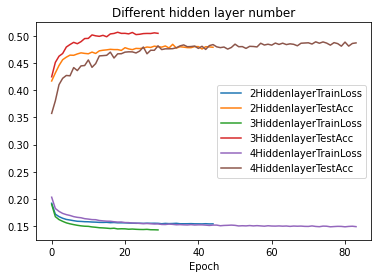
\includegraphics[scale=0.5]{Figures/1.Hiddenlayers/download}
    \caption{Performance of different hidden layer number}
\end{figure}

    As observed, 3 hidden layer obtained both fast training and higher accuracy.

\subsection{Batch Size}

\subsection{Preprocessing}

\subsection{Optimizer}

\subsection{Learning Rate}

\subsection{Initialization}

\subsection{Batch Normalization}

\subsection{Dropout}

\section{Discussion}\label{sec:discussion}


\section{Conclusion}\label{sec:conclusion}


\section{Appendix}\label{sec:appendix}


\end{document}